\documentclass[10pt,lualatex]{beamer}

\usefonttheme{professionalfonts}
\usepackage{xltxtra}	% XeLaTeX
\usepackage{float}
\usepackage{graphicx}
\usepackage{wrapfig}	% Wrap text around figs
\usepackage{lscape}
\usepackage{rotating}	% Sideways figure
\usepackage{hyperref}	% Hyperlinks
\usepackage{caption}	% Hyperlinks to float top
\usepackage{subcaption}
\usepackage{units}		% dB unit
\usepackage[a4paper,width=150mm,top=25mm,bottom=25mm]{geometry}	% margins
\usepackage{tikz}
\usepackage[section]{placeins}	% Don't let floats float before sections
\usepackage{listings}
\usepackage{amsmath}  % align equations
\usepackage{biblatex}

\usepackage{fancyhdr} % headers-footers
\usepackage{mathtools}
% Tables
\usepackage{array}
\usepackage{booktabs}
% for having numbers aligned to the decimal point
\usepackage{siunitx}


%-------------------------------------Custom commands----------------------------------------------------------
  \usepackage{amsfonts}
  \def \IN{\mathbb N} \def \IZ{\mathbb Z} \def \IQ{\mathbb Q} \def \IR{\mathbb R} \def \IC{\mathbb C}
  \def \NN{\mathbb N} \def \ZZ{\mathbb Z} \def \QQ{\mathbb Q} \def \RR{\mathbb R} \def \CC{\mathbb C}
%-------------------------------GREEK LETTERS DEFINITION-------------------------------------------------------
  \newcommand{\gra}{{\alpha}} \newcommand{\grb}{{\beta}} \newcommand{\grg}{{\gamma}} \newcommand{\grd}{{\delta}}
  \newcommand{\gre}{{\epsilon}} \newcommand{\grz}{{\zeta}} \newcommand{\grh}{{\eta}} \newcommand{\gru}{{\theta}}
  \newcommand{\gri}{{\iota}} \newcommand{\grk}{{\kappa}} \newcommand{\grl}{{\lambda}} \newcommand{\grm}{{\mu}}
  \newcommand{\grn}{{\nu}} \newcommand{\grj}{{\xi}} \newcommand{\gro}{{\rm o}} \newcommand{\grp}{{\pi}}
  \newcommand{\grr}{{\rho}} \newcommand{\grs}{{\sigma}} \newcommand{\grt}{{\tau}} \newcommand{\gry}{{\upsilon}}
  \newcommand{\grf}{{\phi}} \newcommand{\grx}{{\chi}} \newcommand{\grc}{{\psi}} \newcommand{\grv}{{\omega}}
  \newcommand{\grA}{{\rm A}} \newcommand{\grB}{{\rm B}} \newcommand{\grG}{{\Gamma}} \newcommand{\grD}{{\Delta}}
  \newcommand{\grE}{{\rm E}} \newcommand{\grZ}{{\rm Z}} \newcommand{\grH}{{\rm H}} \newcommand{\grU}{{\Theta}}
  \newcommand{\grI}{{\rm I}} \newcommand{\grK}{{\rm K}} \newcommand{\grL}{{\Lambda}} \newcommand{\grM}{{\rm M}}
  \newcommand{\grN}{{\rm N}} \newcommand{\grJ}{{\Xi}} \newcommand{\grO}{{\rm O}} \newcommand{\grP}{{\Pi}}
  \newcommand{\grR}{{\rm R}} \newcommand{\grS}{{\Sigma}} \newcommand{\grT}{{\rm T}} \newcommand{\grY}{{\rm Y}}
  \newcommand{\grF}{{\Phi}} \newcommand{\grX}{{\rm X}} \newcommand{\grC}{{\Psi}} \newcommand{\grV}{{\Omega}}
%---------------------------------------------------------------------------------------------------------------

\setromanfont[Mapping=tex-text]{Linux Libertine O}
\setsansfont[Mapping=tex-text]{DejaVu Sans}
\setmonofont[Mapping=tex-text]{DejaVu Sans Mono}

%\geometry{margin=2.5cm}
\pagestyle{fancy}

\graphicspath{ {figures/} }
\addbibresource{references.bib}

% Alignment and placing of subtables
%   https://tex.stackexchange.com/questions/294589/alignment-and-placing-of-subtables
\usepackage{booktabs,subcaption,amsfonts,dcolumn}
\newcolumntype{d}[1]{D..{#1}}
\newcommand\mc[1]{\multicolumn{1}{c}{#1}} % handy shortcut macro

\renewcommand{\figurename}{Σχήμα}
\renewcommand{\tablename}{Πίνακας}
\renewcommand{\contentsname}{Περιεχόμενα}

\usetikzlibrary{arrows.meta,automata,decorations.pathmorphing,decorations.markings,
  backgrounds,positioning,fit,shapes.misc,
  graphs,arrows
}
\tikzset{node/.style={
    rectangle,
    minimum size= 1.2cm,
    thick, draw=black,
    top color=white!50!yellow!10!,
    bottom color=yellow!50!white!50!,
    font=\ttfamily
}}

\usepackage{fancybox}
\usepackage{minibox}
%\usepackage[backend=biber, style=numeric, citestyle=authoryear]{biblatex}
\usepackage[absolute,overlay]{textpos}
\usetheme{metropolis}
\graphicspath{ {../figures/},{../design_walkthrough/build/} }

\definecolor{light-gray}{gray}{0.22}
\usepackage{../jlcode}
%\lstset{columns=fullflexible,numbersep=0pt,resetmargins= true}

\usepackage{minted}
\usemintedstyle{paraiso-dark}
%\usemintedstyle{lovelace}
%\usemintedstyle{friendly}
\setmonofont{Everson Mono}

\defbeamertemplate{description item}{align left}{\insertdescriptionitem\hfill}

\setbeamercolor{framesource}{fg=gray}
\setbeamerfont{framesource}{size=\tiny}
\newcommand{\source}[1]{\begin{textblock*}{4cm}(0.3cm,8.6cm)
    \begin{beamercolorbox}[ht=0.5cm,left]{framesource}
        \usebeamerfont{framesource}\usebeamercolor[fg]{framesource} Πηγή: {#1}
    \end{beamercolorbox}
\end{textblock*}}


%---		BIBLIOGRAPHY		---%
\addbibresource{../references.bib}
\addbibresource{../extra_refs/primary.bib}
\addbibresource{../extra_refs/secondary.bib}
%\setbeamertemplate{bibliography item}[text]
\renewcommand*{\bibfont}{\footnotesize}

\newcommand{\titlestring}{Υψηλού επιπέδου υλοποίηση των αλγορίθμων Hierarchical Temporal Memory σε Julia}
\newcommand{\authorstring}{Κωνσταντίνος Σαμαράς-Τσακίρης}
\hypersetup{%
    pdfencoding=auto,
    pdfauthor={\authorstring},
    pdftitle={\titlestring}
    }

\title{\huge{\titlestring}}
\author{\authorstring\\
Επιβλέπων καθηγητής: Νίκος Πιτσιάνης}
\date{13 Ιουνίου 2019}


\begin{document}

\begin{frame}%{\maketitle}
  \titlepage
\end{frame}

\begin{frame}{Για τι θα μιλήσουμε;}
	\begin{block}{Περίληψη της εργασίας}
		\scriptsize
		\justifying
    Παρουσιάζεται μια αλγοριθμική θεωρία της νοημοσύνης εν τη γενέσει, η \textbf{Hierarchical Temporal Memory} (HTM).
    \alert{\small Βασικοί αλγόριθμοι της θεωρίας υλοποιούνται σε υψηλού επιπέδου γλώσσα με εκφραστική περιεκτικότητα, τη Julia,
    για την καταπολέμηση της υψηλής \textbf{γλωσσικής πολυπλοκότητας}\parencite{chazelleNaturalAlgorithmsInfluence}} (δυσκολίας στην περιγραφή).
    \alert{\small Η προγραμματιστική διατύπωση των αλγορίθμων παραμένει κοντά στην πηγαία μαθηματική διατύπωση,}
    διευκολύνοντας τη μετέπειτα ανάλυση και τον πειραματισμό με νέες αλγοριθμικές ιδέες και προεκτάσεις.
    Η HTM είναι βιολογικά περιορισμένη θεωρία, που αποσκοπεί καταρχήν στην εξήγηση της λειτουργίας του νεοφλοιού (εγκεφαλική δομή)
    και μόνο κατ'επέκτασιν σε εφαρμογές τεχνητής νοημοσύνης.
    Οι υλοποιήσεις σε Julia περιγράφονται αναλυτικά.
    Επαληθεύονται με τις υλοποιήσεις αυτές βασικές ιδιότητες των αλγορίθμων, εν είδει ελέγχου ορθότητας.
    Εν τέλει, προτείνονται κατευθύνσεις έρευνας στην HTM που διευκολύνονται από την παρούσα εργασία.
    Κορωνίδα του έργου είναι η \textit{δημοσίευση πακέτου ανοιχτού λογισμικού} που υλοποιεί τους βασικούς αλγορίθμους HTM σε Julia.
	\end{block}
	\pause
	\begin{itemize}
		\item Πώς η πρότυπη υλοποίηση\\
		1450 γραμμών κώδικα $\longrightarrow$ 340 γραμμές υψηλού επιπέδου
	\end{itemize}
\end{frame}

\section{Hierarchical Temporal Memory}

\begin{frame}{Νευρώνας}
  \centering
	\begin{figure}[h]
		\begin{subfigure}{0.30\textwidth}
			\includesvg[width=\textwidth]{../figures/pyramidal_cell.svg}
		\end{subfigure}
		\hfill
		\begin{subfigure}{0.65\textwidth}
			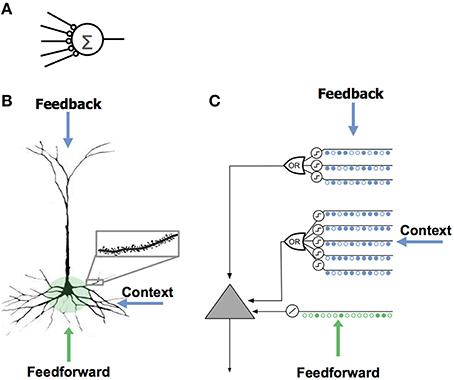
\includegraphics[width=\textwidth]{../figures/numenta_neuron}
		\end{subfigure}
	\end{figure}
	\source{\parencite{wiki_pyramidalcell,hawkinsWhyNeuronsHave2016}}
\end{frame}

\begin{frame}{Μικροστήλες}
  \centering
  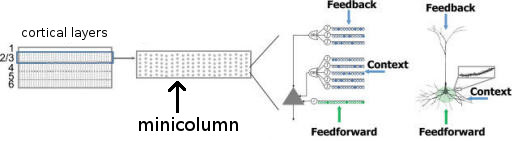
\includegraphics[width=.85\textwidth]{../figures/layer-minicolumn}
  \source{\parencite{cuiContinuousOnlineSequence2016}}
\end{frame}

\begin{frame}{Φλοιικές στήλες}
  \centering
  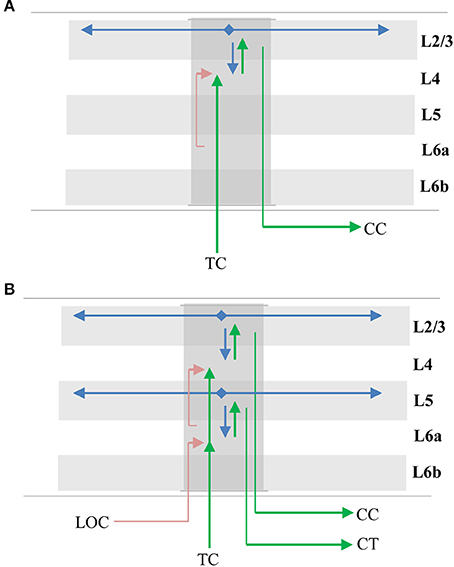
\includegraphics[width=.6\textwidth]{../figures/layers_in_column}
  \source{\parencite{hawkinsTheoryHowColumns2017}}
\end{frame}

\begin{frame}{Αναστολή μεταξύ μικροστηλών}
  \centering
  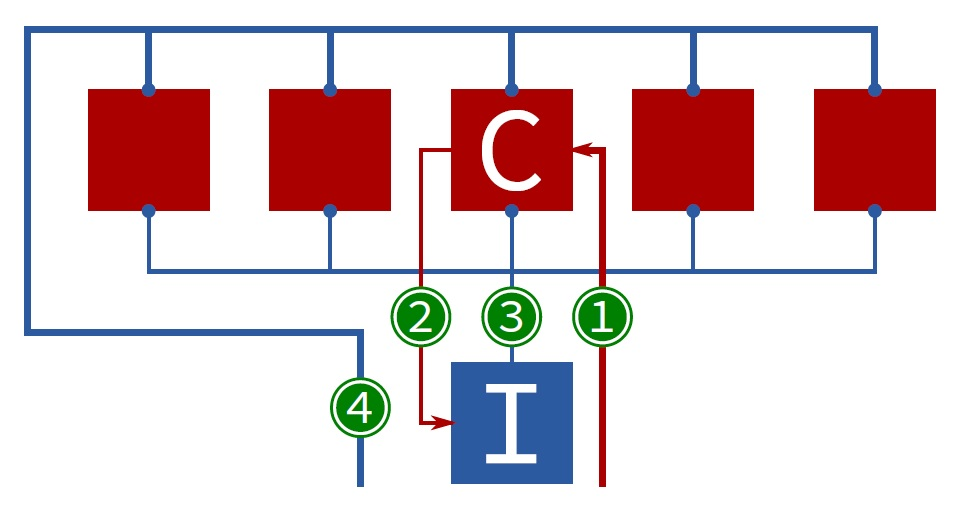
\includegraphics[width=.85\textwidth]{../figures/spatial_hardware}
  \source{\parencite{billaudellePortingHTMModels2015}}
\end{frame}

\begin{frame}{Χωρικός συγκεντρωτής}
  \only<1>{
  \centering
  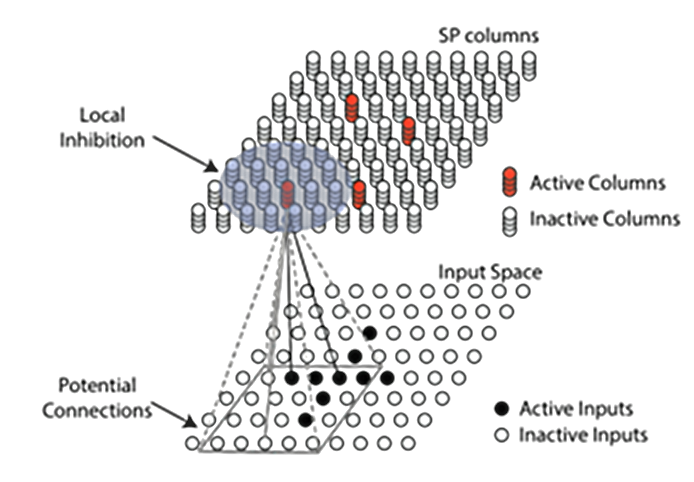
\includegraphics[width=.7\textwidth]{../figures/vlsi-present/spatpool}
  \source{\parencite{cuiHTMSpatialPooler2017}}
  }
  \only<2->{
  \begin{columns}
    \column{0.5\textwidth}
    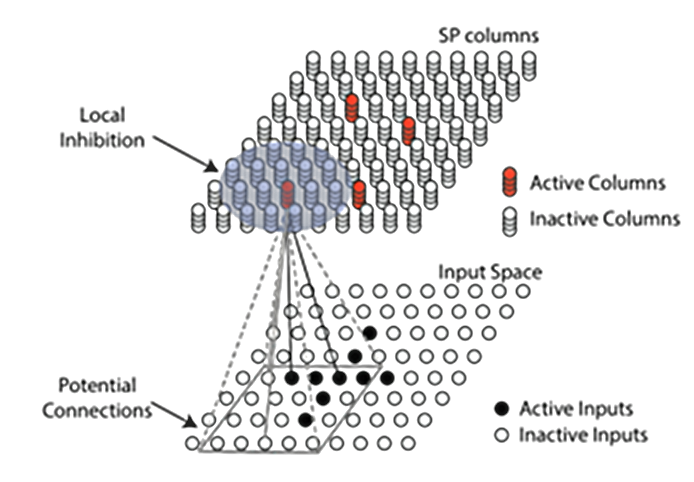
\includegraphics[width=1.15\textwidth]{../figures/vlsi-present/spatpool}
    \begin{block}{Μεταβλητές κατάστασης}
      \small
      \begin{description}[dggg]
        \item[$\mathbf{D_p}$] $∈ 𝕊𝕢^{\mathit{Νᵢₙ×Nₛₚ}}$ πίνακας συναπτικών μονιμοτήτων
        \item[$\hat{a}ₜ$] $∈ 𝔹^{Nₛₚ}$ μεση δραστηριότητα μικροστηλών
      \end{description}
    \end{block}
    \source{\parencite{cuiHTMSpatialPooler2017}}
    \column{0.5\textwidth}
    \begin{block}{Βήματα}
      \small
      \begin{enumerate}
        \setcounter{enumi}{-1}
        \item \alert<3>{Αντιστοίχιση χώρων εισόδου/εξόδου, αρχικοποίηση εγγύς συνάψεων}
        \item \alert<3>{Επικάλυψη μικροστηλών με συνδεδεμένες εισόδους}
        \item Παρώθηση
        \item Τοπική αναστολή
        \item Ενεργοποίηση μικροστηλών που νίκησαν
        \item \alert<3>{Εκμάθηση συνάψεων ενεργών μικροστηλών}
      \end{enumerate}
    \end{block}
  \end{columns}
  }
\end{frame}

\section{Στοιχεία Χωρικού Συγκεντρωτή}

\begin{frame}[fragile]{Αντιστοίχιση εισόδου/εξόδου: υπερκύβος}
\begin{block}{Δείκτης υπερκύβου}
  \[ I(x_j; x_i^c, γ) = \mathit{true} \iff x_j \in \text{ hypercube} \]
  \vspace{-2.2\topsep}
  \begin{description}[ddddd]
		\small
    \item[$x^c$] κέντρο υπερκύβου
    \item[$γ$] ακτίνα υπερκύβου
  \end{description}
\end{block}
\pause
\begin{minted}[fontsize=\scriptsize,bgcolor=light-gray,breaklines]{julia}
struct Hypercube{N}
  xᶜ::NTuple{N,Int}
  γ::Int
  sz::NTuple{N,Int}
  indices::CartesianIndices{N}
end
Hypercube(xᶜ,γ,sz)= Hypercube(xᶜ,γ,sz, start(xᶜ,γ,sz))
start(xᶜ,γ,sz)= CartesianIndices(map( (a,b)-> a:b,
                    max.(xᶜ .- γ, 1), min.(xᶜ .+ γ, sz) ))
Base.collect(hc::Hypercube)= map(c->c.I, collect(hc.indices))

jl> collect(Hypercube((1,1),1,(5,5)))
2×2 Array{Tuple{Int64,Int64},2}:
 (1, 1)  (1, 2)
 (2, 1)  (2, 2)
\end{minted}
\end{frame}

\begin{frame}[fragile]{Αρχικοποίηση συνάψεων}
\begin{onlyenv}<1-2>
\begin{block}{Εν δυνάμει συνδέσεις}
  \[ Π_i= \{j \;|\, I(x_j; x_i^c, γ) \wedge Z_{ij} < p\} \]
  όπου $Ζ \in U(0,1)$ τυχαίος αριθμός
\end{block}
\pause
\begin{minted}[fontsize=\footnotesize,bgcolor=light-gray,breaklines]{julia}
c2lᵢₙ= LinearIndices(szᵢₙ)
c2lₛₚ= LinearIndices(szₛₚ)

Dₚ= zeros(𝕊𝕢, prod(szᵢₙ),prod(szₛₚ))
foreach(out_lattice()) do yᵢ
  # Linear indices from hypercube
  x= @>> yᵢ xᶜ xᵢ collect map(x->c2lᵢₙ[x...])
  Dₚ[x, c2lₛₚ[yᵢ...]]= permanences(@> yᵢ xᶜ xᵢ)
end

@> yᵢ xᶜ xᵢ === xᵢ(xᶜ(yᵢ))
\end{minted}
\end{onlyenv}

\only<3>{
\begin{figure}
  \includegraphics[width=\textwidth]{../design_walkthrough/build/figures/sp_design_15_1.pdf}
\end{figure}
}
\end{frame}

\begin{frame}[fragile]{Επικάλυψη}
\begin{block}{Επικάλυψη μικροστηλών με συνδεδεμένες εισόδους}
  \begin{align*}
    \mathbf{W} &= \mathbf{D_p} \ge θ_c\\
    o &= b\:\mathbf{W}'z
  \end{align*}
  %\setbeamertemplate{description item}[align left]
  \vspace{-2.2\topsep}
  \begin{description}[ddddd]
		\small
	  \item[$\mathbf{W}$] [$ℓ_{in} × ℓ_{sp}$] συνδεδεμένες συνάψεις
	  \item[$z$] [$ℓ_{in}$] είσοδος
	  \item[$b$] [$ℓ_{sp}$] παρώθηση
  \end{description}
\end{block}
\pause
\begin{columns}[T]
\column{0.6\textwidth}
\begin{minted}[fontsize=\footnotesize,bgcolor=light-gray,breaklines]{julia}
Wₚ()= Dₚ .≥ θ_permanence
o(z)= @> (b() .* Wₚ()'z) reshape(szₛₚ)
\end{minted}
\pause
\column{0.4\textwidth}
\begin{block}{broadcasting}
\begin{minted}[fontsize=\footnotesize,bgcolor=light-gray,breaklines]{julia}
f(x::Int)= x+1;
jl> f.([1; 10; 100])
3-element Array{Int64,1}:
   2
  11
 101
\end{minted}
\end{block}
\end{columns}
\end{frame}

\begin{frame}[fragile]{Εκμάθηση συνάψεων}
\begin{block}{Κανόνας πλαστικότητας τύπου Hebbian (\footnotesize STDP, spike-timing-dependent-plasticity)}
  \[ \mathbf{ΔD_p} = p^+(z◦\mathbf{D_p}◦c) - p^-(\lnot z◦ \mathbf{D_p}◦c)\]
	όπου $c$ αποτέλεσμα του $z$.
  \begin{description}[fffff]
		\small
    \item[$c$] ενεργοποίηση χωρικού συγκεντρωτή
  \end{description}
\end{block}
\begin{onlyenv}<2>
\begin{block}{Απλούστερος τρόπος}
\begin{minted}[fontsize=\footnotesize,bgcolor=light-gray,breaklines]{julia}
learn!(Dₚ,z,a)= begin
  Dₚ[z,a]  .= (Dₚ[z,a].>0) .* (Dₚ[z,a]   .⊕ p⁺)
  Dₚ[.!z,a].= (Dₚ[z,a].>0) .* (Dₚ[.!z,a] .⊖ p⁻)
end
\end{minted}
\end{block}
\end{onlyenv}
\begin{onlyenv}<3>
\begin{block}{Καλύτερα}
\begin{minted}[fontsize=\footnotesize,bgcolor=light-gray,breaklines]{julia}
learn!(Dₚ,z,a)= begin
  Dₚactive= @view Dₚ[:,a]   # the only elements we touch
  activeConn=   (Dₚactive .> 0) .&   z
  inactiveConn= (Dₚactive .> 0) .& .!z
  Dₚactive.= activeConn   .* (Dₚactive .⊕ p⁺) .+
             inactiveConn .* (Dₚactive .⊖ p⁻)
end
\end{minted}
\end{block}
\end{onlyenv}
\end{frame}

\section{Χρονική μνήμη}

\begin{frame}{Αναστολή \alert{εντός} μικροστηλών}
  \centering
  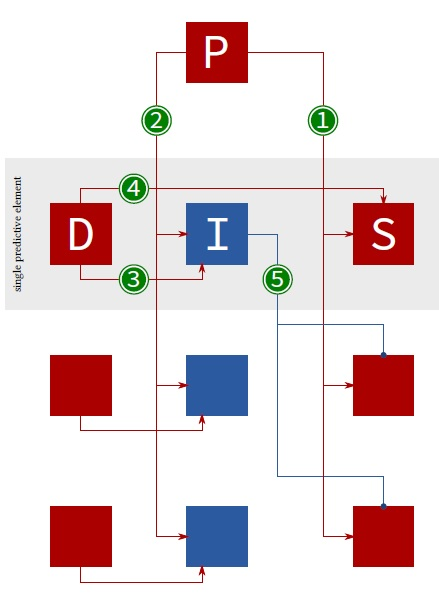
\includegraphics[width=.5\textwidth]{../figures/temporal_hardware}
  \source{\parencite{billaudellePortingHTMModels2015}}
\end{frame}

\begin{frame}{Μνήμη ακολουθιών}
  \centering
  \only<1>{
  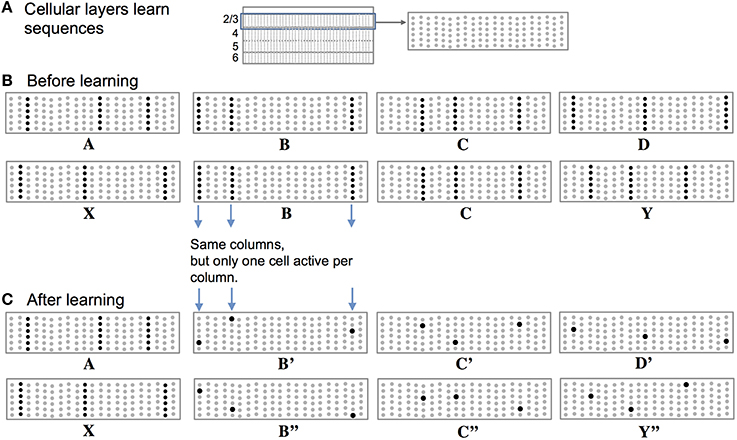
\includegraphics[width=\textwidth]{../figures/numenta_temporal_memory1}
	\source{\parencite{hawkinsWhyNeuronsHave2016}}

		Μνήμη ανώτερης τάξης
  }
  \only<2-3>{
  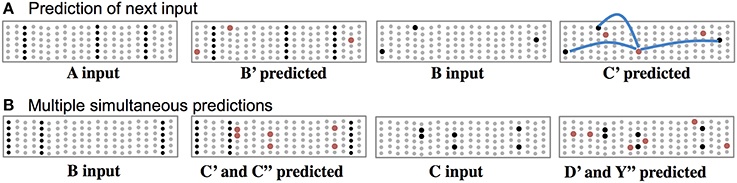
\includegraphics[width=\textwidth]{../figures/numenta_temporal_memory2}
	\source{\parencite{hawkinsWhyNeuronsHave2016}}
		\vspace{-1em}
		Αναπαράσταση αμφιβολίας
  \pause
  \begin{columns}[T]
    \column{0.4\textwidth}
    \begin{block}{Βήματα}
      \small
      \begin{enumerate}
      \item \alert<3>{Ενεργοποίηση}
      \item Προσδοκία/πρόβλεψη
			\item Υπολογισμός νικητών νευρώνων \& δενδριτών
      \item \alert<3>{Εκμάθηση συνάψεων ενεργών νευρώνων}
      \end{enumerate}
    \end{block}
    \column{0.6\textwidth}
		\pause
    \begin{block}{Μεταβλητές κατάστασης}
			\small
      \begin{description}[ddddd]
        \item[$\mathbf{D_d}$] $∈ 𝕊𝕢^{\mathit{Nₙ×Nₛ}}$ \alert{αραιός} πίνακας συναπτικών μονιμοτήτων\\
				[προσυναπτικοί νευρώνες {\large×} μετασυναπτικοί δενδρίτες]
        \item[$\mathbf{NS}$] $∈ 𝔹^{\mathit{Nₙ×Nₛ}}$ πίνακας γειτνίασης νευρώνων - δενδριτών
        \item[$\mathbf{SC}$] $∈ 𝔹^{\mathit{Nₛ×N_c}}$ πίνακας γειτνίασης δενδριτών - μικροστηλών
      \end{description}
    \end{block}
  \end{columns}
  }
	\only<4>{
		\begin{figure}
		  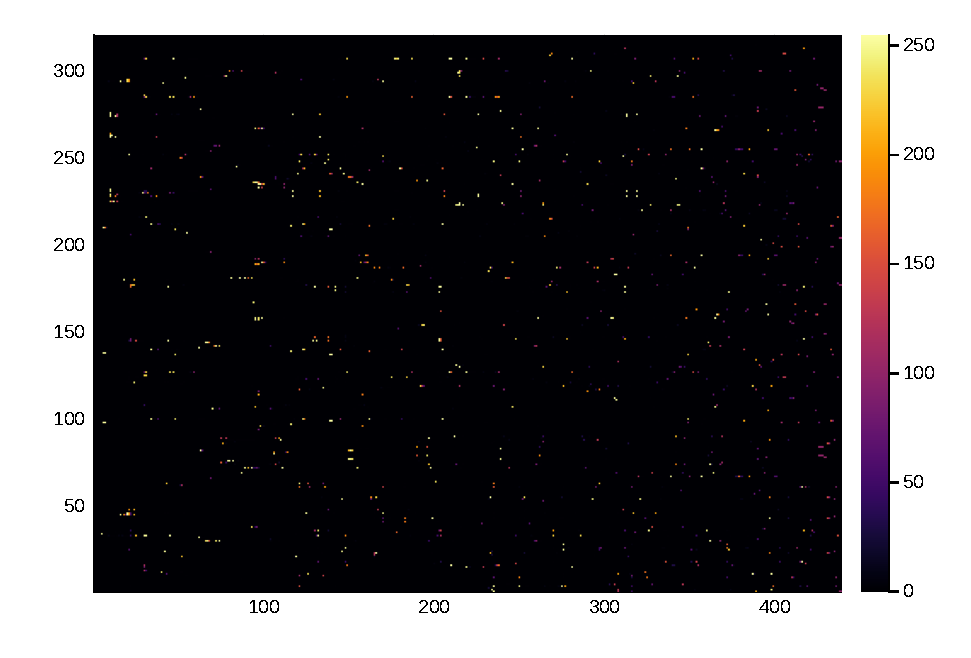
\includegraphics[width=\textwidth]{../figures/distalSynapses_learned}
		\end{figure}
	}
\end{frame}

\begin{frame}[fragile]{Ενεργοποίηση χρονικής μνήμης}
\begin{block}{Ενεργοποίηση}
  \begin{equation}
    α_{ij}= \begin{cases} 1, &j \in c \:\wedge\: π_{ij}^{t-1}=1 \text{ (πρόβλεψη)}\\
                          1, &j \in c \:\wedge\: \sum_i π_{ij}^{t-1}=0 \text{ (έξαρση)}\\
                          0, &\text{ αλλιώς}
            \end{cases}
  \end{equation}
  \begin{description}[fffff]
    \item[$c$] ενεργές μικροστήλες
    \item[$π_{ij}$] προβλεπτικοί νευρώνες, j: μικροστήλη, i: νευρώνας στη j
  \end{description}
\end{block}
\begin{minted}[fontsize=\footnotesize,bgcolor=light-gray,breaklines]{julia}
burst(c,Π)= c .& .!@percolumn(any,Π, k)
predicted(c,Π)= @percolumn(&,Π,c, k)
activate(c,Π)= (predicted(c,Π) .| burst(c,Π)')|> vec
\end{minted}
\end{frame}

\begin{frame}[fragile]{Εκμάθηση συνάψεων}
\begin{onlyenv}<1>
\begin{block}{Κανόνας πλαστικότητας τύπου Hebbian {\small (αντίστοιχος με ΧΣ)}}
  \[ \mathbf{ΔD_d} = p^+(α^{t-1}◦\mathbf{D_d}◦\mathit{WS}) \;-\; p^-(\lnot α^{t-1}◦ \mathbf{D_d}◦\mathit{WS}) \]
  \vspace{-1.0\topsep}
  \begin{description}[fffff]
		\item[$α$] ενεργοί νευρώνες
    \item[$\mathit{WS}$] «νικητές» δενδρίτες: $\in π^{t-1} \;\cap\; α^t$
  \end{description}
\end{block}

Διατρέχοντας τον αραιό (CSC) $\mathbf{D_d}$ κατά στήλες:
\begin{minted}[fontsize=\footnotesize,bgcolor=light-gray,breaklines]{julia}
function learn_sparsesynapses(synapses_activeCol,input_i,z,p⁺,p⁻)
  z_i= z[input_i]
  synapses_activeCol.= z_i .* (synapses_activeCol .⊕ p⁺) .+
                     .!z_i .* (synapses_activeCol .⊖ p⁻)
end
sparse_foreach((scol,cell_i)->
                  learn_sparsesynapses(scol,cell_i, pα, p⁺,p⁻),
               D_d, WS)
\end{minted}
\end{onlyenv}
\only<2>{
\begin{figure}
  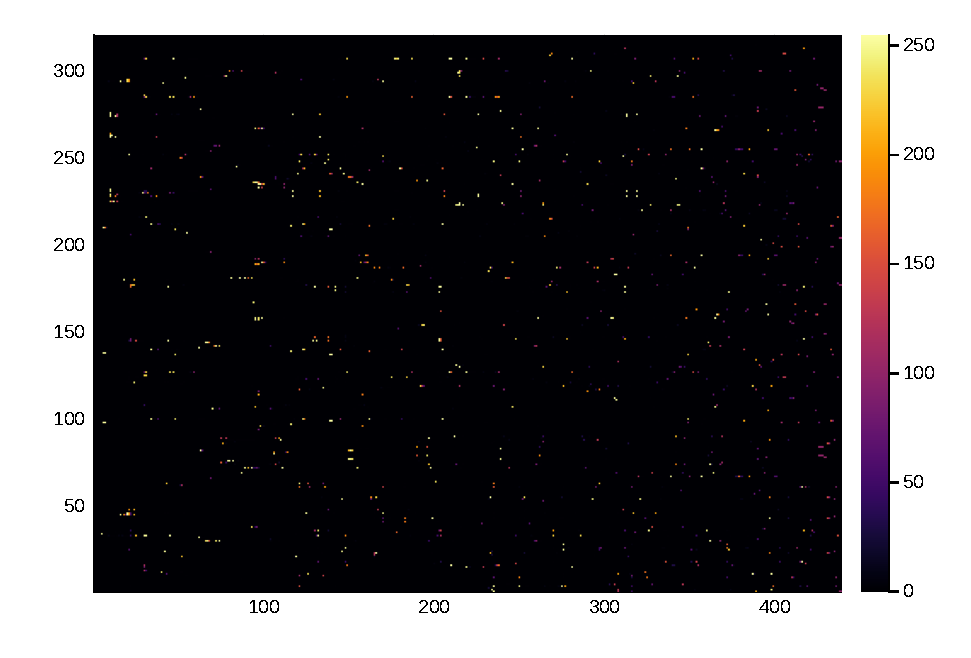
\includegraphics[width=\textwidth]{../figures/distalSynapses_learned}
\end{figure}
}
\end{frame}

\section{Πείραμα πρόβλεψης χρονοσειράς}

\begin{frame}
  \centering
  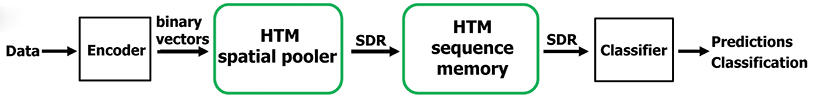
\includegraphics[width=\textwidth]{../figures/htm_predict_pipeline}
  \source{\parencite{cuiHTMSpatialPooler2017}}
  \pause
  \begin{figure}
    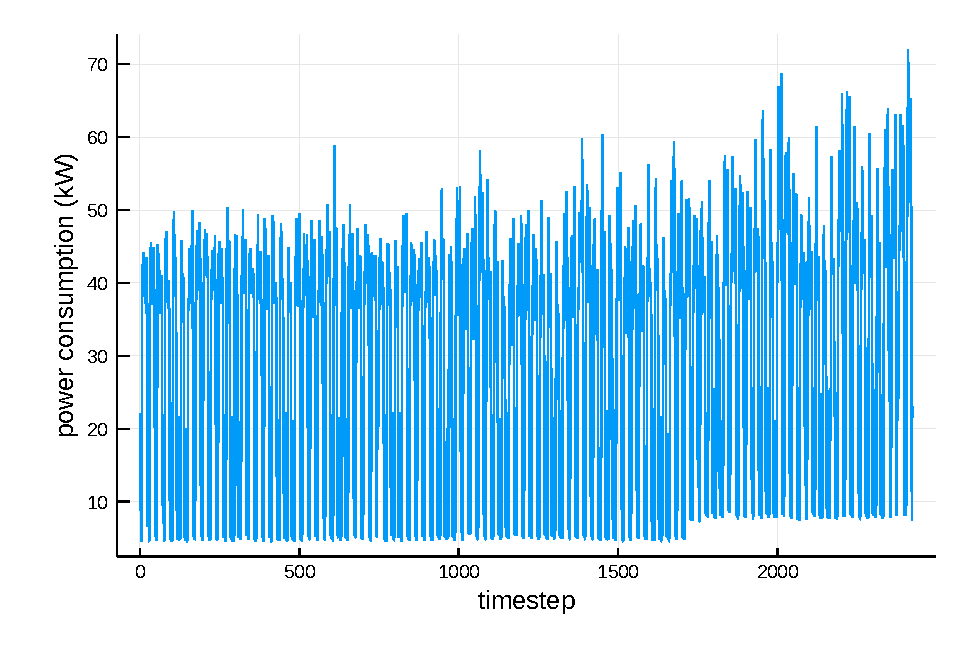
\includegraphics[width=\textwidth,height=6cm]{../figures/tshotgym}
    \caption{Ωριαία κατανάλωση ισχύος σε γυμναστήριο}
  \end{figure}
\end{frame}

\begin{frame}{Πρόβλεψη 1 στιγμή μπροστά}
  \centering
  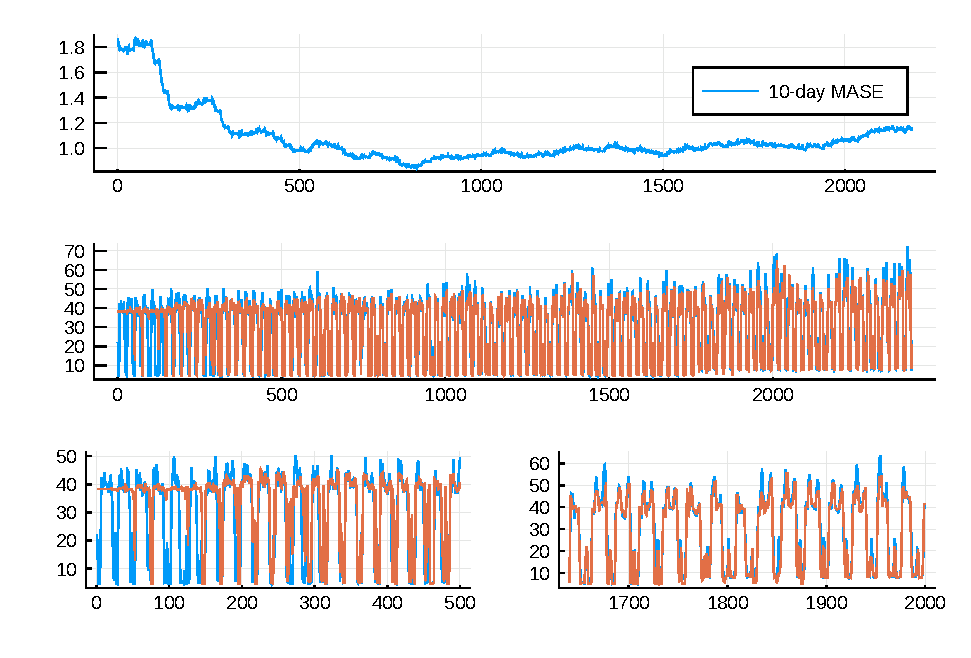
\includegraphics[width=\textwidth]{../figures/tm1.eps}
\end{frame}

\begin{frame}{Προτάσεις για μελέτη στην HTM}
    \alert{Χρονική συγκέντρωση}. Πόλωση από την προσδοκώμενη ακολουθία \cite{hawkinsTheoryHowColumns2017}

    Συνένωση πολλών περιοχών σε \alert{ιεραρχικό μοντέλο} \cite{hawkinsFrameworkIntelligenceCortical2019}

		Μελέτη κανόνων εκμάθησης από οπτικη \alert{θεωρίας γράφων} \cite{kipouridisConvergenceNetworkSystems2019}
\end{frame}

\begin{frame}[plain,allowframebreaks]
  \printbibliography[title=Βιβλιογραφία]
\end{frame}

\section{Παράρτημα}
\begin{frame}{Διατήρηση ομοιότητας από χωρικό συγκεντρωτή}
	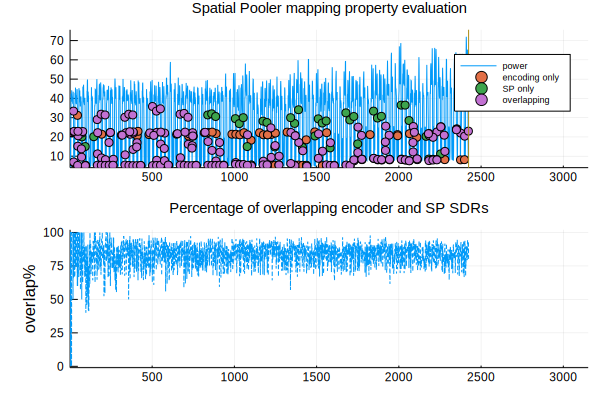
\includegraphics[width=\textwidth]{../figures/sp3}
\end{frame}

\end{document}
